\documentclass[twocolumn,10pt]{jarticle}
\setlength{\columnsep}{3zw}
\usepackage{color}
\usepackage[dvipdfmx]{graphicx}
\usepackage{amsmath,amssymb}
\usepackage[linesnumbered,ruled,vlined]{algorithm2e}
\usepackage{bm}
\usepackage[top=10truemm,bottom=20truemm,left=15truemm,right=15truemm]{geometry}


% LaTeXについてはこちらを参考にして下さい.
% http://mikilab.doshisha.ac.jp/dia/seminar/latex/index.html

\title{中間発表}
\author{名前:松浦隆斗}
\date{日付: 11/24}

\begin{document}
\maketitle

%箇条書き
%\begin{itemize}
%      \item TeXでの参考文献の引用方法\cite{DE}.
%      \item 複数の文献を引用する\cite{EA1,EA2}.
%\end{itemize}
\section{後期までに行ったこと}
ε制約法のεレベルの制御は、あらかじめ決まっているスケジュールで制御していくので、個体群の進化度合いなどを考慮していない点から、εレベルの制御を個体群の動きに依存させるようにし、改善を試みた。
また、ベースベクトルの選択方法の変更や、探索終盤でのパラメータ変更による改良を狙う。

\section{はじめに}
\subsection{進化的アルゴリズム(Evolutionary Algorithm, EA)}
進化的アルゴリズムとは、生物が子孫繁栄するシステムを模倣し、最適解を探索する最適化アルゴリズムである。

\subsection{Differential Evolution(DE)}
DEは、親個体と子個体から得られる情報により、任意で決定するパラメータを用いて繰り返し解の改良を行い最適解を探索するアルゴリズムである。アルゴリズムの実装は容易だが、最適解がパラメータの値ごとに大きく違ってくる場合もある。パラメータは初期に決定するのは困難であり、DEは制約付き最適化問題を直接解くことが出来ない。そこで、今回はεレベル比較を使用するε制約法を導入したεDEをベースアルゴリズムとする。
DEの表記は、DE/base/num/crossで、baseはベースベクトル$\bm{x}_{r1}$の選択方法、numはベースベクトルを変異させるための差分ベクトルの個数、crossは、交叉方法をそれぞれ指定する。εDEの戦略も通常のDEと同様に表記するので、εDE/base/num/crossとして表記される。今回は、ベースベクトルの選択をrand戦略でnum=1とし、交叉を2項交叉(binomial crossover)とするεDE/rand/1/binのアルゴリズムである。

\subsection{例:DEアルゴリズム(DE/rand/1)}
DEのシステムの例をあげる。
(DE/rand/1)の場合では、集団内の各個体がターゲットベクトル$\bm{x}_{i}$(親)として順番に選択される。$\bm{x}_{i}$に対して、個体集団からベースベクトル$\bm{x}_{r1}$と差分生成のための2個体($\bm{x}_{r2}$,$\bm{x}_{r3}$)を選択する。ここで、$\bm{x}_{r1}$,$\bm{x}_{r2}$,$\bm{x}_{r3}$は集団からランダムに選択し、重複はないものとする。$\bm{x}_{r1}$,$\bm{x}_{r2}$,$\bm{x}_{r3}$を使い、突然変異を行い変異ベクトル$\bm{v}_{i}$を生成し、ターゲットベクトル$\bm{x}_{i}$と変異ベクトル$\bm{v}_{i}$を交叉することによりトライアルベクトル$\bm{u}_{i}$を生成する。最後に生存選択をし親と子の結果を比較して良い方を選択する。これを集団サイズ分繰り返し行い、次の世代の探索を行う。


\subsection{マツダベンチマーク問題}
DEなどのアルゴリズムを実行するときの対象問題として解かれるのがベンチマーク問題である。ベンチマーク問題は、人工的に作成された問題である場合があり、もし良い結果が得られたとしても、実問題に対して良い結果が得られるとは限らないと言える。そこで、実問題として提案されたのがマツダベンチマーク問題である。マツダベンチマーク問題は、車の車体総重量の最小化と共通板厚部品点数の最大化の2目的の制約付き最適化問題である。また、解の評価回数は30000回となっている。

\section{複数車種の同時最適化問題(マツダベンチマーク問題)}
マツダベンチマーク問題は、等式制約を含まない不等式制約条件付き多目的最適化問題であり、目的関数は車の総重量の最小化と共通板厚部品数の最大化となる。本研究では、車の総重量の最小化のみを目的とする単目的ベンチマーク問題とし、以下のように定義する。\\
\\
{\large{Design Variables:}}
\begin{eqnarray}
\bm{x}_{SUV}=\bm{(\bm{x}_1,\bm{x}_2,...,\bm{x}_d)}^T,\\
\bm{x}_{CDW}=\bm{(\bm{x}_{1+d},\bm{x}_{2+d},...,\bm{x}_{2d})}^T,\\
\bm{x}_{C5H}=\bm{(\bm{x}_{1+2d},\bm{x}_{2+2d},...,\bm{x}_{3d})}^T,\\
d=74,=3d\nonumber
\end{eqnarray}
\\
{\large{Minimize:}}
\begin{eqnarray}
\bm{f}_1=Mass(\bm{x}_{SUV})+Mass(\bm{x}_{CDW})+Mass(\bm{x}_{C5H})
\end{eqnarray}
\\
{\large{Minimize:}}
\begin{eqnarray}
\bm{g}_j(\bm{x}_{SUV})\geq0,\\
\bm{g}_{P+j}(\bm{x}_{CDW})\geq0,\\
\bm{g}_{2P+j}(\bm{x}_{C5H})\geq0,\\
j=1,2,...,P,P=18\nonumber\\
SUV:\bm{x}^L_i\leq \bm{x}_i\leq \bm{x}^U_i,\\
SDW:\bm{x}^L_i+d\leq \bm{x}_i+d\leq \bm{x}^U_i+d,\\
C5H:\bm{x}^L_i+2d\leq \bm{x}_i+2d\leq \bm{x}^U_i+2d,\\
i=1,2,...,d,\nonumber\\
\bm{x}^L_i=\bm{x}^L_i+d=\bm{x}^L_i+2d,\bm{x}^U_i=\bm{x}^U_i+d=\bm{x}^U_i+2d
\end{eqnarray}
$\bm{f}_1$は最小化すべき目的関数であり、車格の異なる3車種、SUV-Car(SUV),Large-Car,Small-Carの総重量である。設計変数ベクトルxの要素数Dは3d=222になる。設計要件上の変数の大小関係に関する制約関数と、各車種ごとに応答局面法で算出するk=54種類の制約関数が存在する。$\bm{x}^L_i$,$\bm{x}^U_i$(i=1,2,...,D)は設計変数の下限値、上限値である。さらに、以下でがすべての制約を満足する領域を実行可能解F、上下限制限を満足する領域を探索空間Sとする。


\section{ε制約法}
\subsection{制約逸脱度}
ε制約法では、制約をどの程度逸脱しているかを表現するために、制約逸脱度φ(x)を導入する。制約逸脱度φ(x)は、以下を満足する関数である。Fは実行可能状態。
\begin{eqnarray}
\left\{
\begin{array}{cc}
    \bm{φ(x)}=0(x\in{F})\\
    \bm{φ(x)}>0(x\notin{F})\\
\end{array}
\right.
\end{eqnarray}
制約逸脱度関数φ(x)には幾つかの定義方法があるが、今回はG(x)をxの制約逸脱度ベクトルとし、φ(x)は以下のように制約総逸脱度として定義する。
\begin{eqnarray}
%\begin{split}
\bm{G(x)}=({G}_1(\bm{x}),\bm{G}_2(x),...,\bm{G}_k(x))\\   
\bm{G}_i(x)=
\left\{
\begin{array}{cc}
     \bm|{g}_i(x)| & \mbox{if${g}_i(x)<0(i=1,2,...,k)$} \\
    \bm{0} & \mbox{otherwise}\\
\end{array}
\right.\\
\bm{φ(x)}=\sum_{i=1}^k \bm{G}_i(x)
%\end{split}
\end{eqnarray}

\subsection{εレベル比較}
目的関数値Fと制約逸脱度φ(x)の改善について、各制約ごとのε制約${ε}_t$を使用し決める。各制約に対する個体ごとに制約違反量g(x)を求め、ε制約と比較し、全ての違反量がε以下の場合は目的関数値の大小関係を優先し、それ以外の場合は制約逸脱度の大小関係を優先する比較であるεレベル比較を定義する。点${x}_1,{x}_2$における関数値を${f}_1,{f}_2$、制約逸脱度を${φ}_1,{φ}_2$とする。定義を以下に示す。
\begin{eqnarray}
\bm({f}_1,{φ}_1){<}_ε({f}_2,{φ}_2)
\leftrightarrow
\left\{
\begin{array}{cc}
    \bm{f}_1<{f}_2 & \mbox{if${φ}_1,{φ}_2 \leq ε$}\\
    \bm{f}_1<{f}_2 & \mbox{if${φ}_1={φ}_2$}\\
    \bm{φ}_1<{φ}_2 & \mbox{otherwise}\\
\end{array}
\right.
\end{eqnarray}
\begin{eqnarray}
\bm({f}_1,{φ}_1){\leq}_ε({f}_2,{φ}_2)
\leftrightarrow
\left\{
\begin{array}{cc}
    \bm{f}_1\leq{f}_2 & \mbox{if${φ}_1,{φ}_2 \leq ε$}\\
    \bm{f}_1\leq{f}_2 & \mbox{if${φ}_1={φ}_2$}\\
    \bm{φ}_1<{φ}_2 & \mbox{otherwise}\\
\end{array}
\right.
\end{eqnarray}
なお、${<}_0,{\leq}_0$は制約逸脱度を優先する辞書式比較と一致し、${<}_∞,{\leq}_∞$は目的関数値のみの比較と一致する。

\subsection{εレベルの制御 兼 提案手法}
εレベルを制御制御する際には、そのレベル以下の個体が常にある程度含まれるようにしながら0まで減少させ、0になった後もある程度の最適化を行うことが望ましい。そこで、初期値$ε(0)$を初期集団の制約逸脱度の良い個体の上位${NP}×s(\bm{s}\in[0,1])$番目の個体の制約逸脱度とし、$\bm{T}_0(0<{T}_0<{T}_{max})$世代以降は常に0となるよう制御する。よって、以下の世代tのべき乗関数による制御方法を用い減少させていく。

\begin{eqnarray}
\bm{ε}(0)=φ({x}_θ)
\end{eqnarray}

\begin{eqnarray}
\bm{ε}(t)=
\left\{
\begin{array}{cc}
    \bm{ε}(0){(1-\frac{t}{T}_0)}^{cp} & \mbox{$0<t<{T}_0$} \\
    \bm{0} & \mbox{$t\geq{T}_0$}\\
\end{array}
\right.
\end{eqnarray}
\\
\\
イメージしやすいように画像をいれる。
\\
\\
今までのε制約法のεレベル制御では、εレベルの初期値は、ある一個体の制約逸脱度から与えられているが、初期値以降になれば、一定のパラメータによってεレベルを減少させスケジューリングがされているため、探索途中における個体集団の制約逸脱度を考慮できていなかったと考える。その点から、εレベルの制御をあらかじめスケジュールを決定するのではなく、各世代で個体集団のある一個体の制約逸脱度をεレベルとすることで、εレベルの制御において常に制約逸脱度を考慮できるようにする。
\\

本研究ではε制約のスケジュールをあらかじめ決定せずに個体群の動きに合わしていくように、各世代における個体群の制約逸脱度の良い個体の上位NP×k番目の制約逸脱度をεレベルに当てはめ制御する。
なお、最終的には制約を違反していない個体が必要となるので、ある世代に到達した時にεレベルを強制的に0とする$\bm{T}_0(0<{T}_0<{T}_{max})$を決めておく。また、εレベルが0になった後もある程度の最適化を行うことが望ましいので、$\bm{T}_0$世代以降は常に0となるように制御する。
よって、以下のように世代tごとでεレベルを制御していく。
\begin{eqnarray}
\bm{ε}(t)=
\left\{
\begin{array}{cc}
    \bm{φ({x}_α)} & \mbox{$0<t<{T}_0$} \\
    \bm{0} & \mbox{$t\geq{T}_0$}\\
\end{array}
\right.
\end{eqnarray}
ここで、${x}_α$は制約逸脱度が上位NP×k番目の個体(α=NP×k)とし、$\bm{T}_0$は$\bm{T}_{max}\times{r}(r\in[0,1])$世代とする。
\\
\\
イメージしやすいように画像をいれる。
\\

\section{ε制約Differential Evolution}
本章では、εレベルの制御を変更したε制約DE(εDE)を説明する。εDEは基本的なアルゴリズムはDEと同様であり、εの制御とεレベル比較を行う点が異なる。また、εDEの戦略も通常のDEと同様に、はεDE/base/num/crossとして表記される。baseはベースベクトル$\bm{x}_{r1}$の選択方法、numはベースベクトルを変異させるための差分ベクトルの個数、crossは交叉方法をそれぞれ指定する。\\
ベースベクトルの選択をrand戦略でnum=1とし、交叉を2項交叉(binomial crossover)とするεDE/rand/1/binのアルゴリズムを以下に示す。
\subsection{初期化}
NP個の初期個体${x}_i$を探索空間S内にランダムに生成し、初期集団P={${x}_i$|i=1,2,...,NP}を構築する。また、ε(0)を与える。
\subsection{終了判定}
終了条件を満たせば、アルゴリズムを終了する。
\subsection{突然変異}
各親個体${x}_i$に対して、3個体{$\bm{x}_{r1}$,$\bm{x}_{r2}$,$\bm{x}_{r3}$}を${x}_i$および互いに重複しないように、個体集団Pからランダムに選択する。その後、式\ref{eq:s1}により変異ベクトル${v}_i$を生成する。
\begin{eqnarray}
\bm{v}_i={x}_{r1}+F({x}_{r2}-{x}_{r3})\\
\label{eq:s1}
\end{eqnarray}
ここで、Fは差分の伸縮を表すスケーリングファクタである。
\subsection{交叉}
変異ベクトル${v}_i$を${x}_i$と交叉し、子個体${u}_i$を生成する。交叉はbinomial crossoverを用いる。式を以下で示す。
\begin{eqnarray}
\bm{u}_j=
\left\{
\begin{array}{cc}
    \bm{u}_j & \mbox{if$({rand}_j[0,1]\leq{C}_R \bigvee j={j}_r)$}\\
    \bm{x}_{j,i,g} & \mbox{$otherwise$}\\
\end{array}
\right.
\end{eqnarray}
${rand}_j$は区間[0,1]の一様乱数であり、${j}_i$は[1,D]区間からランダムに選択した変数番号である。また、CRが大きいほど、変異ベクトルの成分が多くuに受け継がれる。

\subsection{生存選択}
子個体を評価し、親個体${x}_i$とεレベル比較を行う。子個体${u}_i$が親個体${x}_i$よりも良ければ子個体が生存者となり、親を子個体で置換する。
\subsection{εレベルの制御}
εレベル制御関数${ε}_t$によって、εレベルを更新する。
終了判定に戻る。

\section{実験途中結果}
\subsection{実験設定}
本章では、マツダベンチマーク問題に提案手法を適用し、最適化性能と探索の挙動を分析する。目的関数の評価回数の上限は30000回であり、NP=50、最大世代数${T}_{max}$は600世代とした。εレベルの制御のパラメータは、k={0.7,0.8,0.85,0.9}、F=0.2,CR=0.4とした。また、r=0.9とし、それぞれ1試行の実験を行った。

\subsection{提案手法の実験結果}
まず、提案手法を実装していないεDEでパラメータs値を変化させた実験結果を表\ref{tbl:MLP1}に示す。また、ベースベクトルはrand戦略とする。
\begin{table}[htbp]
\begin{center}
\caption{F=0.4,CR=0.9,cp=3,r=0.9,s=0.1,0.2,0.3}
\label{tbl:MLP1}
\begin{tabular}{|l|c|c|}
\hline
s     & 最適解  \\ \hline
s=0.1 & 2.66182	\\ \hline
s=0.2 & 2.64261 \\ \hline
s=0.3 & 2.69370 \\ \hline
\end{tabular}
\end{center}
\end{table}


次に提案手法を実装したεDEでパラメータkの値を変化させた実験結果を表\ref{tbl:MLP2}に示す。また、ベースベクトルはrand戦略とする。

\begin{table}[htbp]
\begin{center}
\caption{F=0.2,CR=0.4,r=0.9,k={0.7,0.8,0.85,0.9}}
\label{tbl:MLP2}
\begin{tabular}{|l|c|c|}
\hline
k     & 最適解  \\ \hline
k=0.7 & 2.68871\\ \hline
k=0.8 & 2.64880\\ \hline
k=0.85 & 2.62735\\ \hline
k=0.9 & 2.57505(実行可能解が得られなかった)\\ \hline
\end{tabular}
\end{center}
\end{table}
上記は良い最適解が得られたパラメータ設定をしている。今回の提案手法であるεレベルの制御を変更し、cpのパラメータを使用せずに比較的同等の結果が得られたといえる。

\subsection{pbest戦略、パレートランク戦略}
この節では、ベースベクトルの戦略を変更することで、提案手法の精度向上を図るためpbest戦略、パレートランク戦略を実装した。実験結果を表\ref{tbl:MLP3}、表\ref{tbl:MLP4}で示す。
\begin{table}[htbp]
\begin{center}
\caption{F=0.2,CR=0.4,r=0.9,k={0.7,0.8,0.85,0.9},pbest戦略,pbest=0.45}
\label{tbl:MLP3}
\begin{tabular}{|l|c|c|}
\hline
k     & 最適解  \\ \hline
k=0.7 & 2.63672\\ \hline
k=0.8 & 2.59544\\ \hline
k=0.85 & 2.58393(実行可能解が得られなかった)\\ \hline
k=0.9 & 2.49864(実行可能解が得られなかった)\\ \hline
\end{tabular}
\end{center}
\end{table}

\begin{table}[htbp]
\begin{center}
\caption{F=0.4,CR=0.5,r=0.9,k={0.7,0.8,0.85,0.9},パレートランク戦略}
\label{tbl:MLP4}
\begin{tabular}{|l|c|c|}
\hline
k     & 最適解  \\ \hline
k=0.7 & 2.64282\\ \hline
k=0.8 & 2.58546\\ \hline
k=0.85 & 2.58749\\ \hline
k=0.9 & 2.58917(実行可能解が得られなかった)\\ \hline
\end{tabular}
\end{center}
\end{table}
上記の表においてパラメータの違いは最適解を得るために変更している。

表\ref{tbl:MLP3}、表\ref{tbl:MLP4}よりパレートランク戦略の方が良い結果が得られた。pbest戦略では、ε制約を満たしている個体の中の目的関数値が良い値の個体から選ぶような、εレベル比較をしているので、ベースベクトルの選択に偏りがでるが、パレートランク戦略では制約逸脱度、目的関数値の両方をバランスよくベースベクトルの選択をできるので良い結果が得られたと考える。また、パレートランク戦略ではpbest戦略のようにパラメータを設定することがないので扱いやすい戦略であり、実問題に対して適していると考える。

\subsection{提案手法でのパラメータkの依存性}
本研究での提案手法では、パラメータcpを使用せず、式(20)のようにパラメータkだけを用いてεレベルの制御をしているので、実行結果がkに大きな影響うける。まず、比較のためk=0.8での個体集団の動きを図\ref{fig2:graph4}、図\ref{fig2:graph5}で示す。次に同じ世代でk=0.5での個体集団の動きを図\ref{fig2:graph6}、図\ref{fig2:graph7}、同じく同じ世代でk=0.9での個体集団の動きを図\ref{fig2:graph8}、図\ref{fig2:graph9}で示す。
\begin{figure}[htbp]
  \centering
  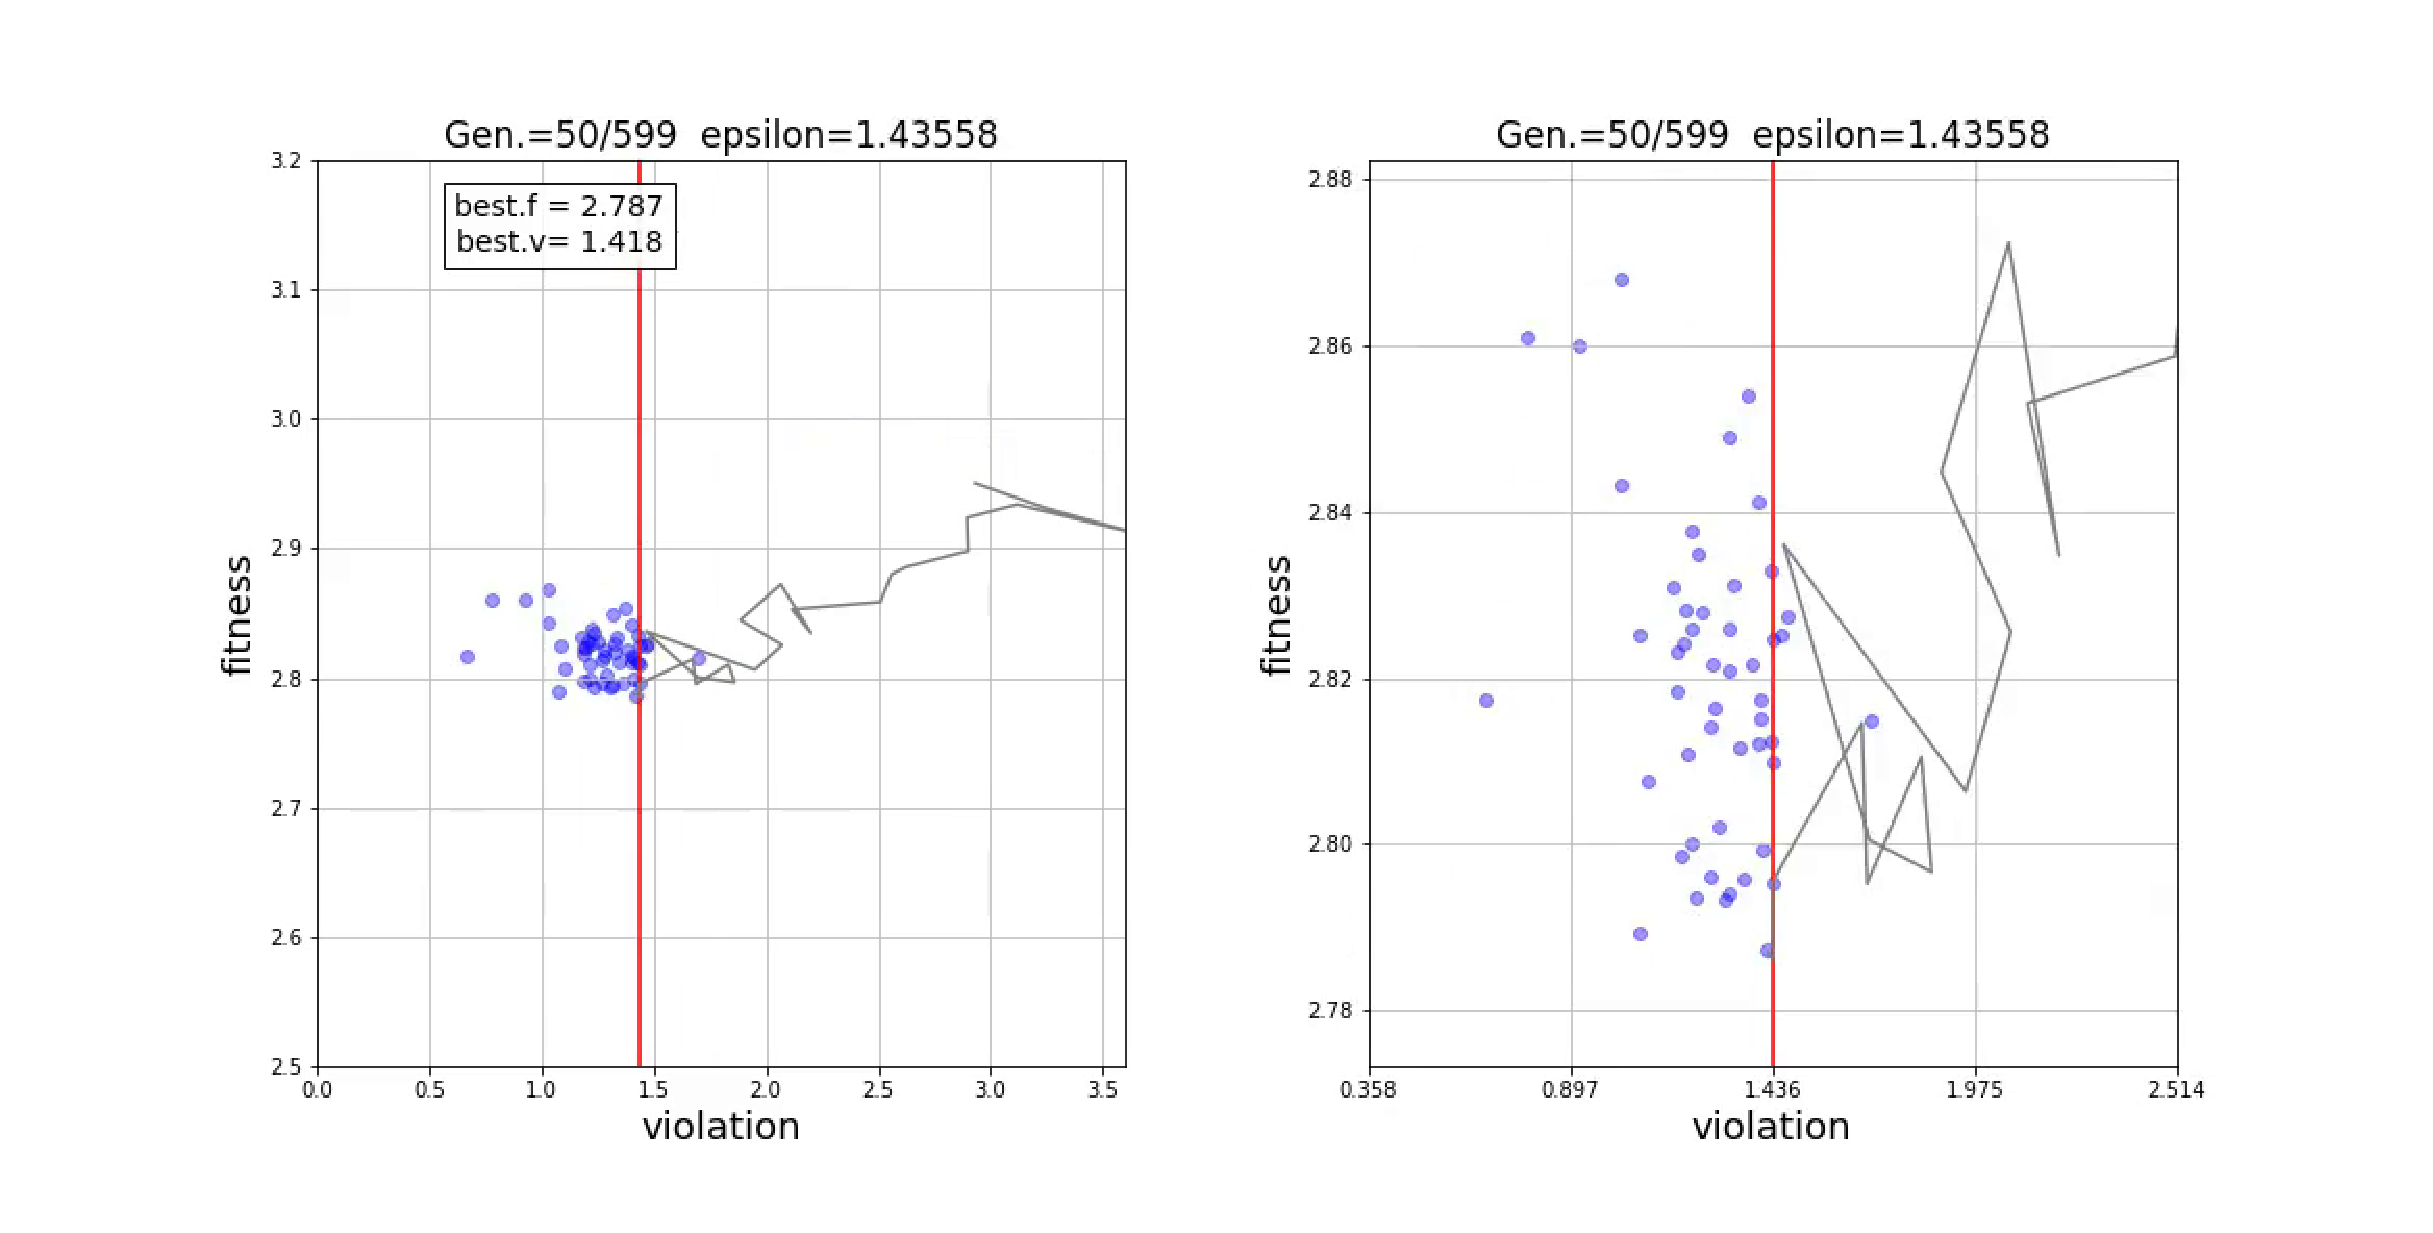
\includegraphics[width=.9\linewidth]{fig2/top_rate=0.8,50.eps}
  \caption{k=0.8,50世代}
\label{fig2:graph4}
\end{figure}
\begin{figure}[htbp]
  \centering
  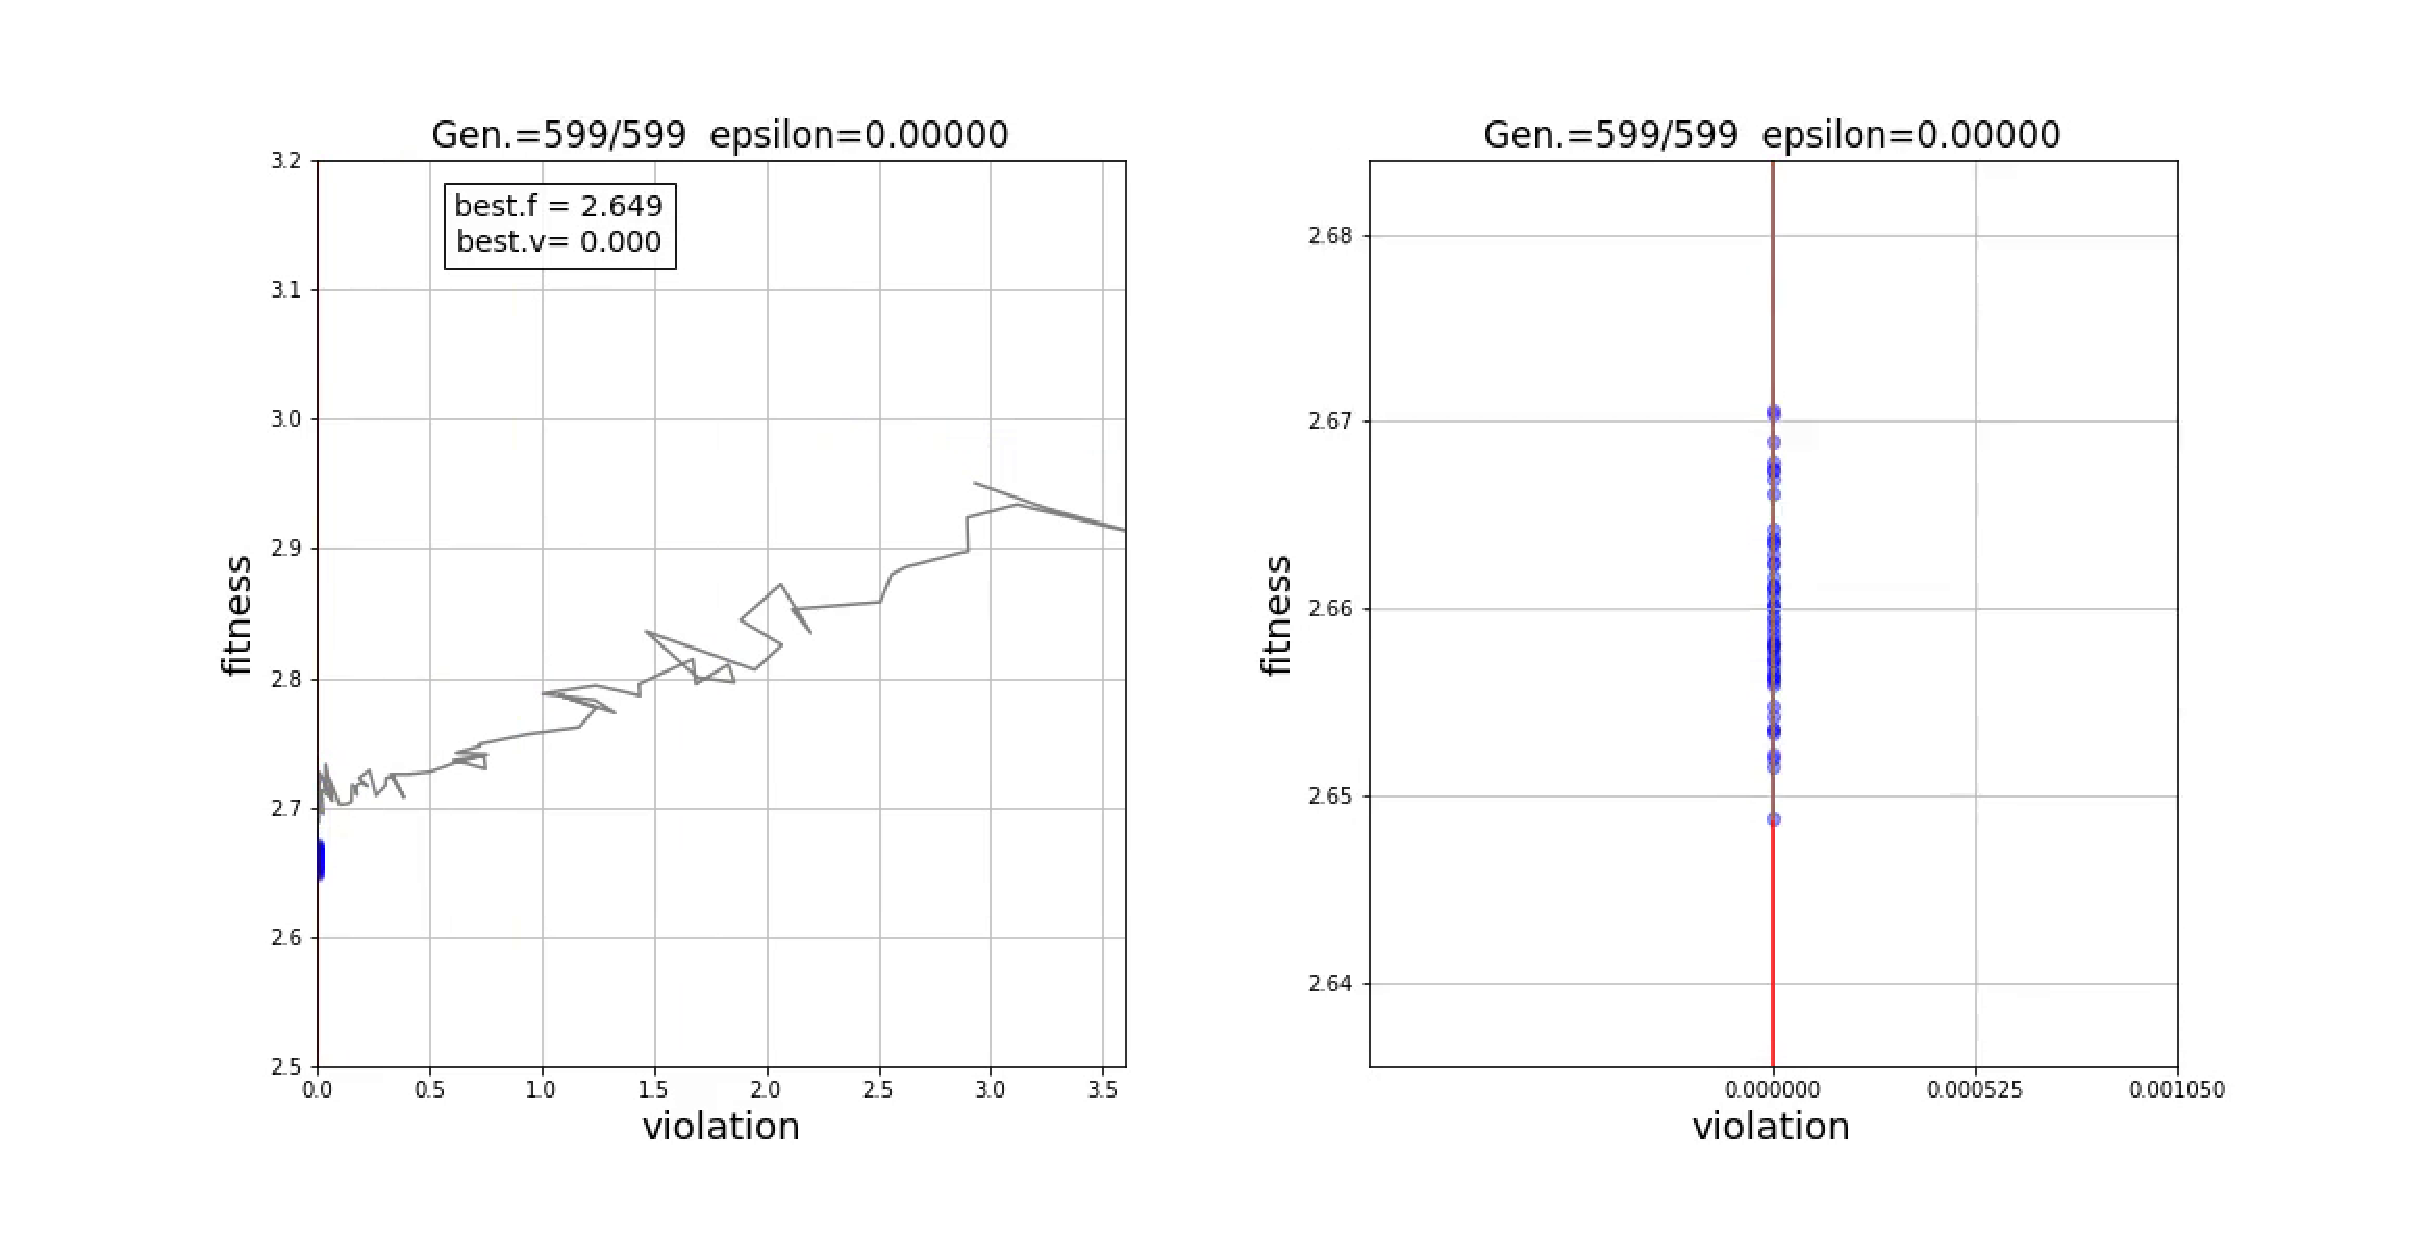
\includegraphics[width=.9\linewidth]{fig2/top_rate=0.8,600.eps}
  \caption{k=0.8、600世代}
\label{fig2:graph5}
\end{figure}
\begin{figure}[htbp]
  \centering
  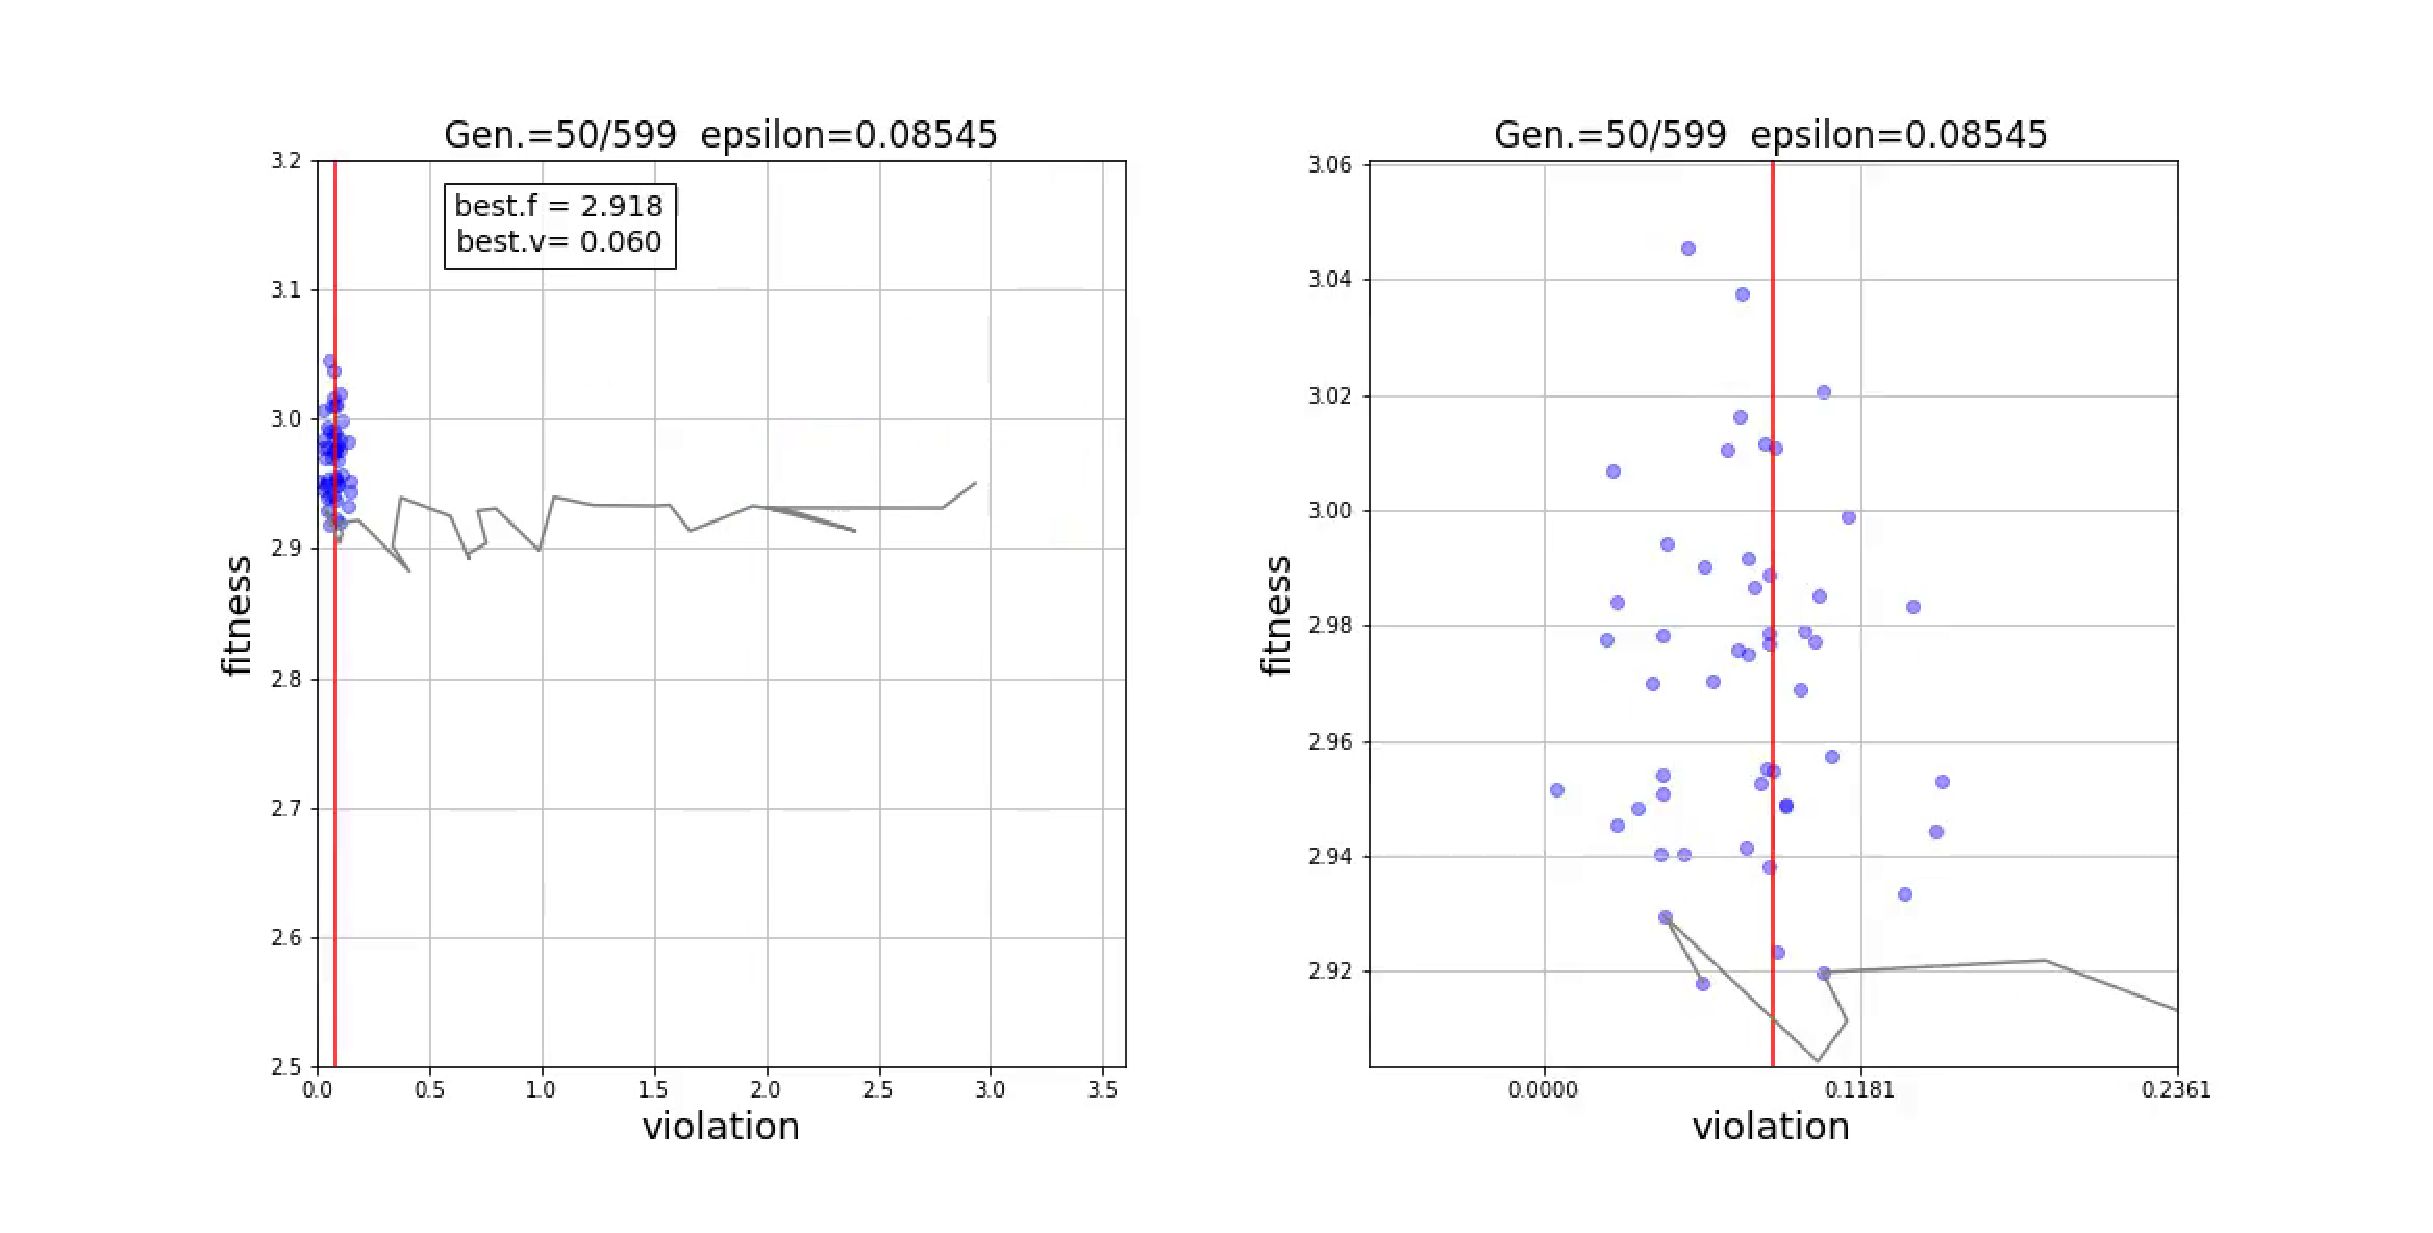
\includegraphics[width=.9\linewidth]{fig2/top_rate=0.5,50.eps}
  \caption{k=0.5,50世代}
\label{fig2:graph6}
\end{figure}
\begin{figure}[htbp]
  \centering
  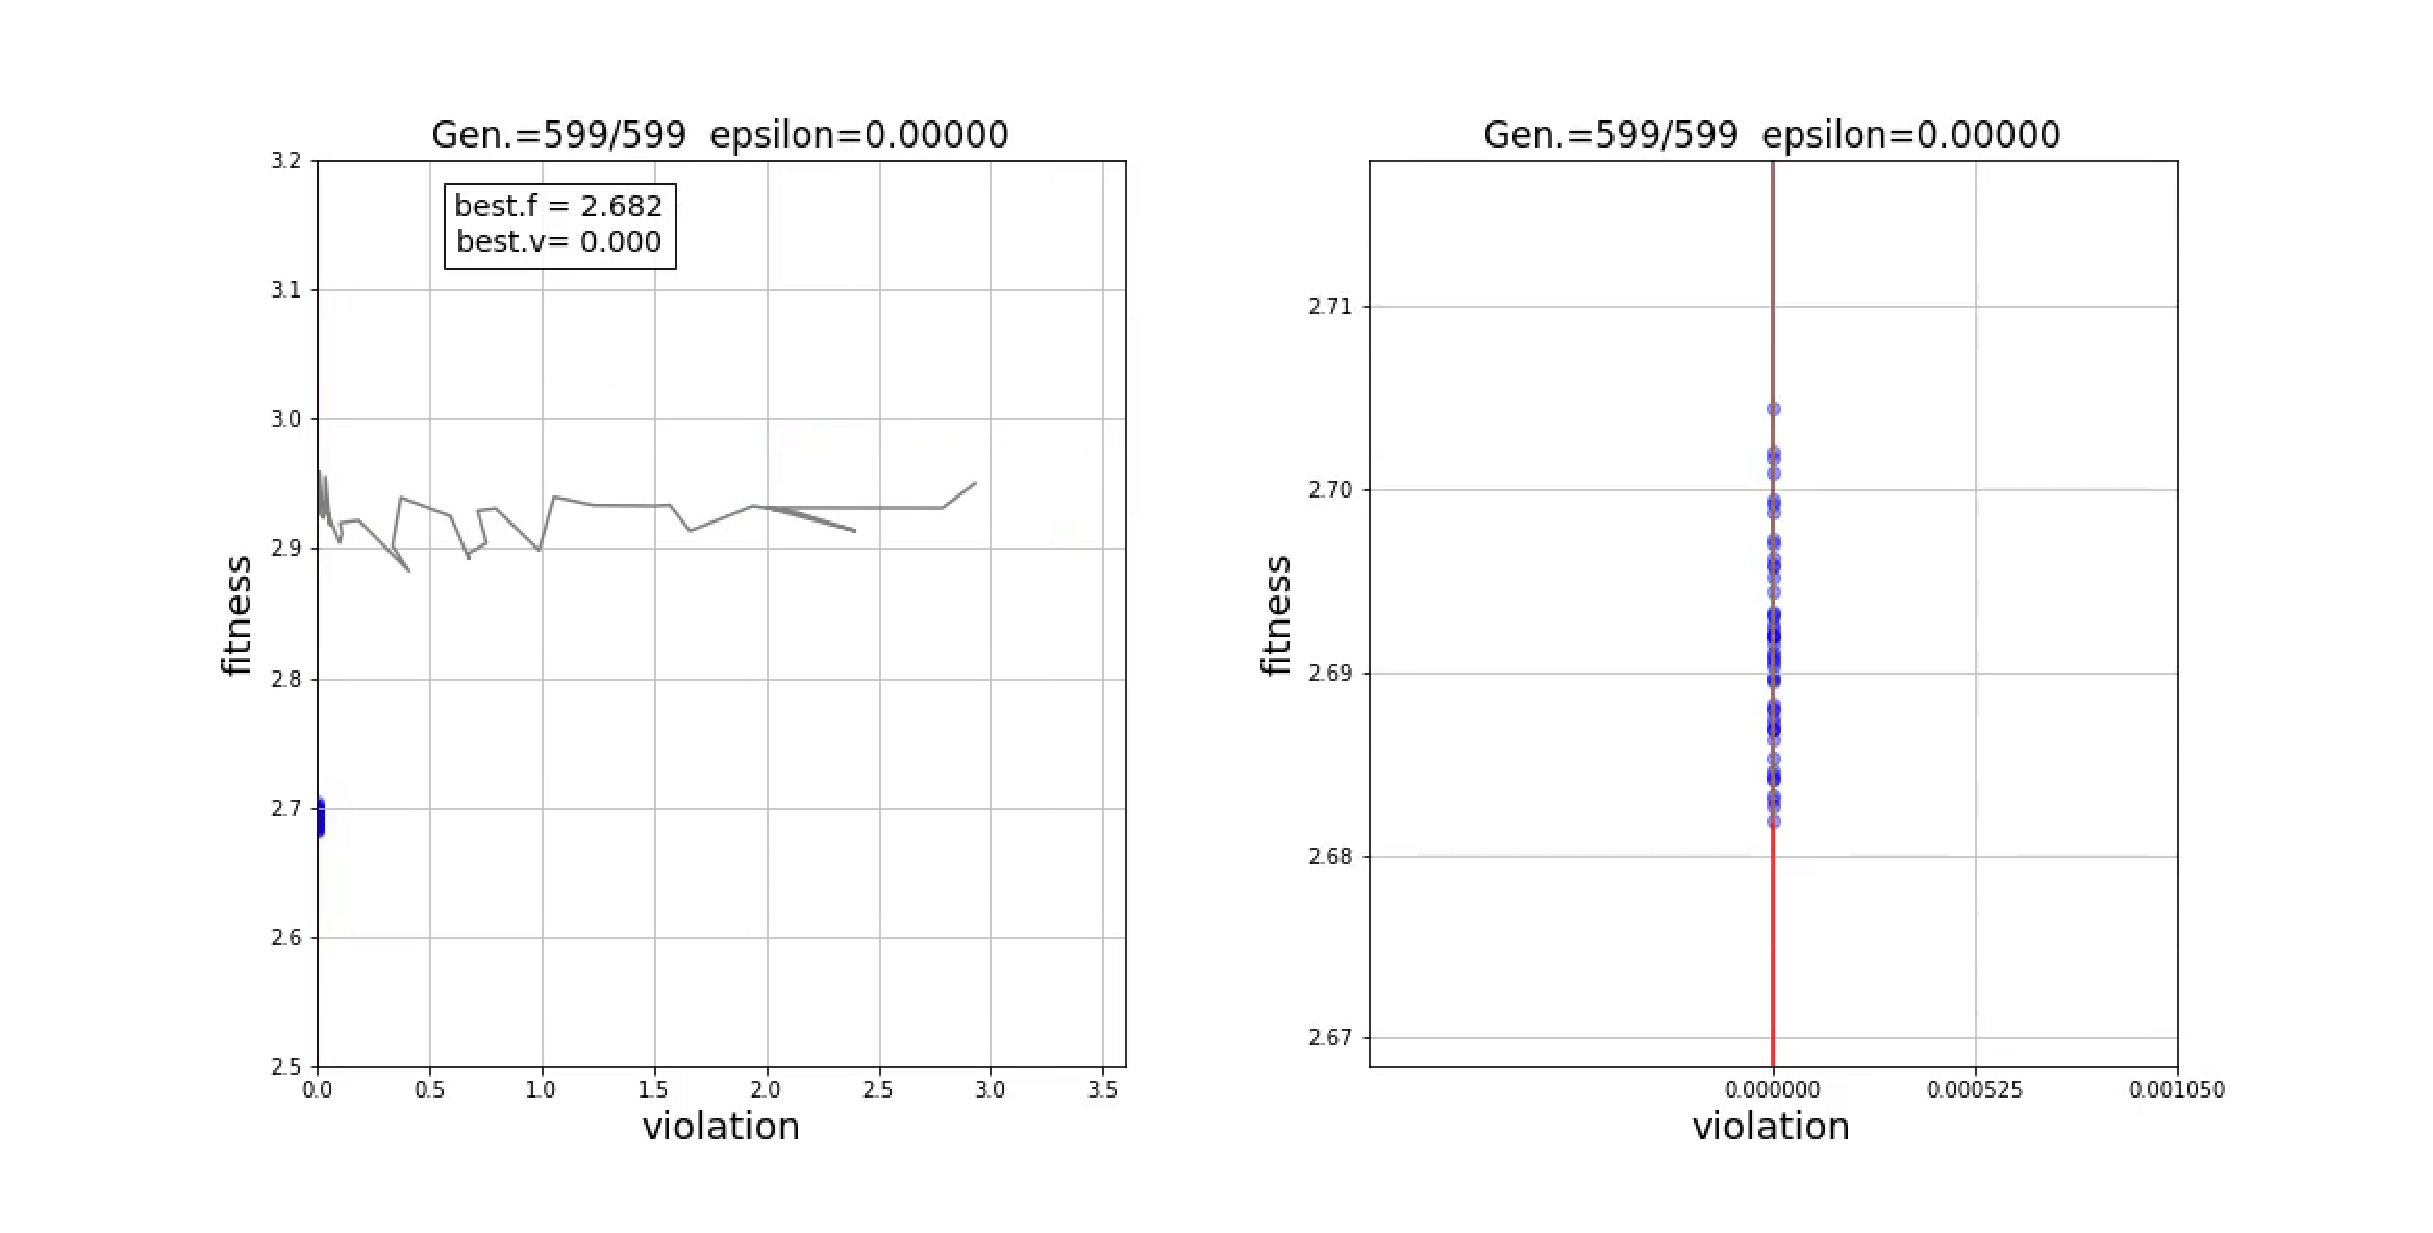
\includegraphics[width=.9\linewidth]{fig2/top_rate=0.5,600.eps}
  \caption{k=0.5,600世代}
\label{fig2:graph7}
\end{figure}
\begin{figure}[htbp]
  \centering
  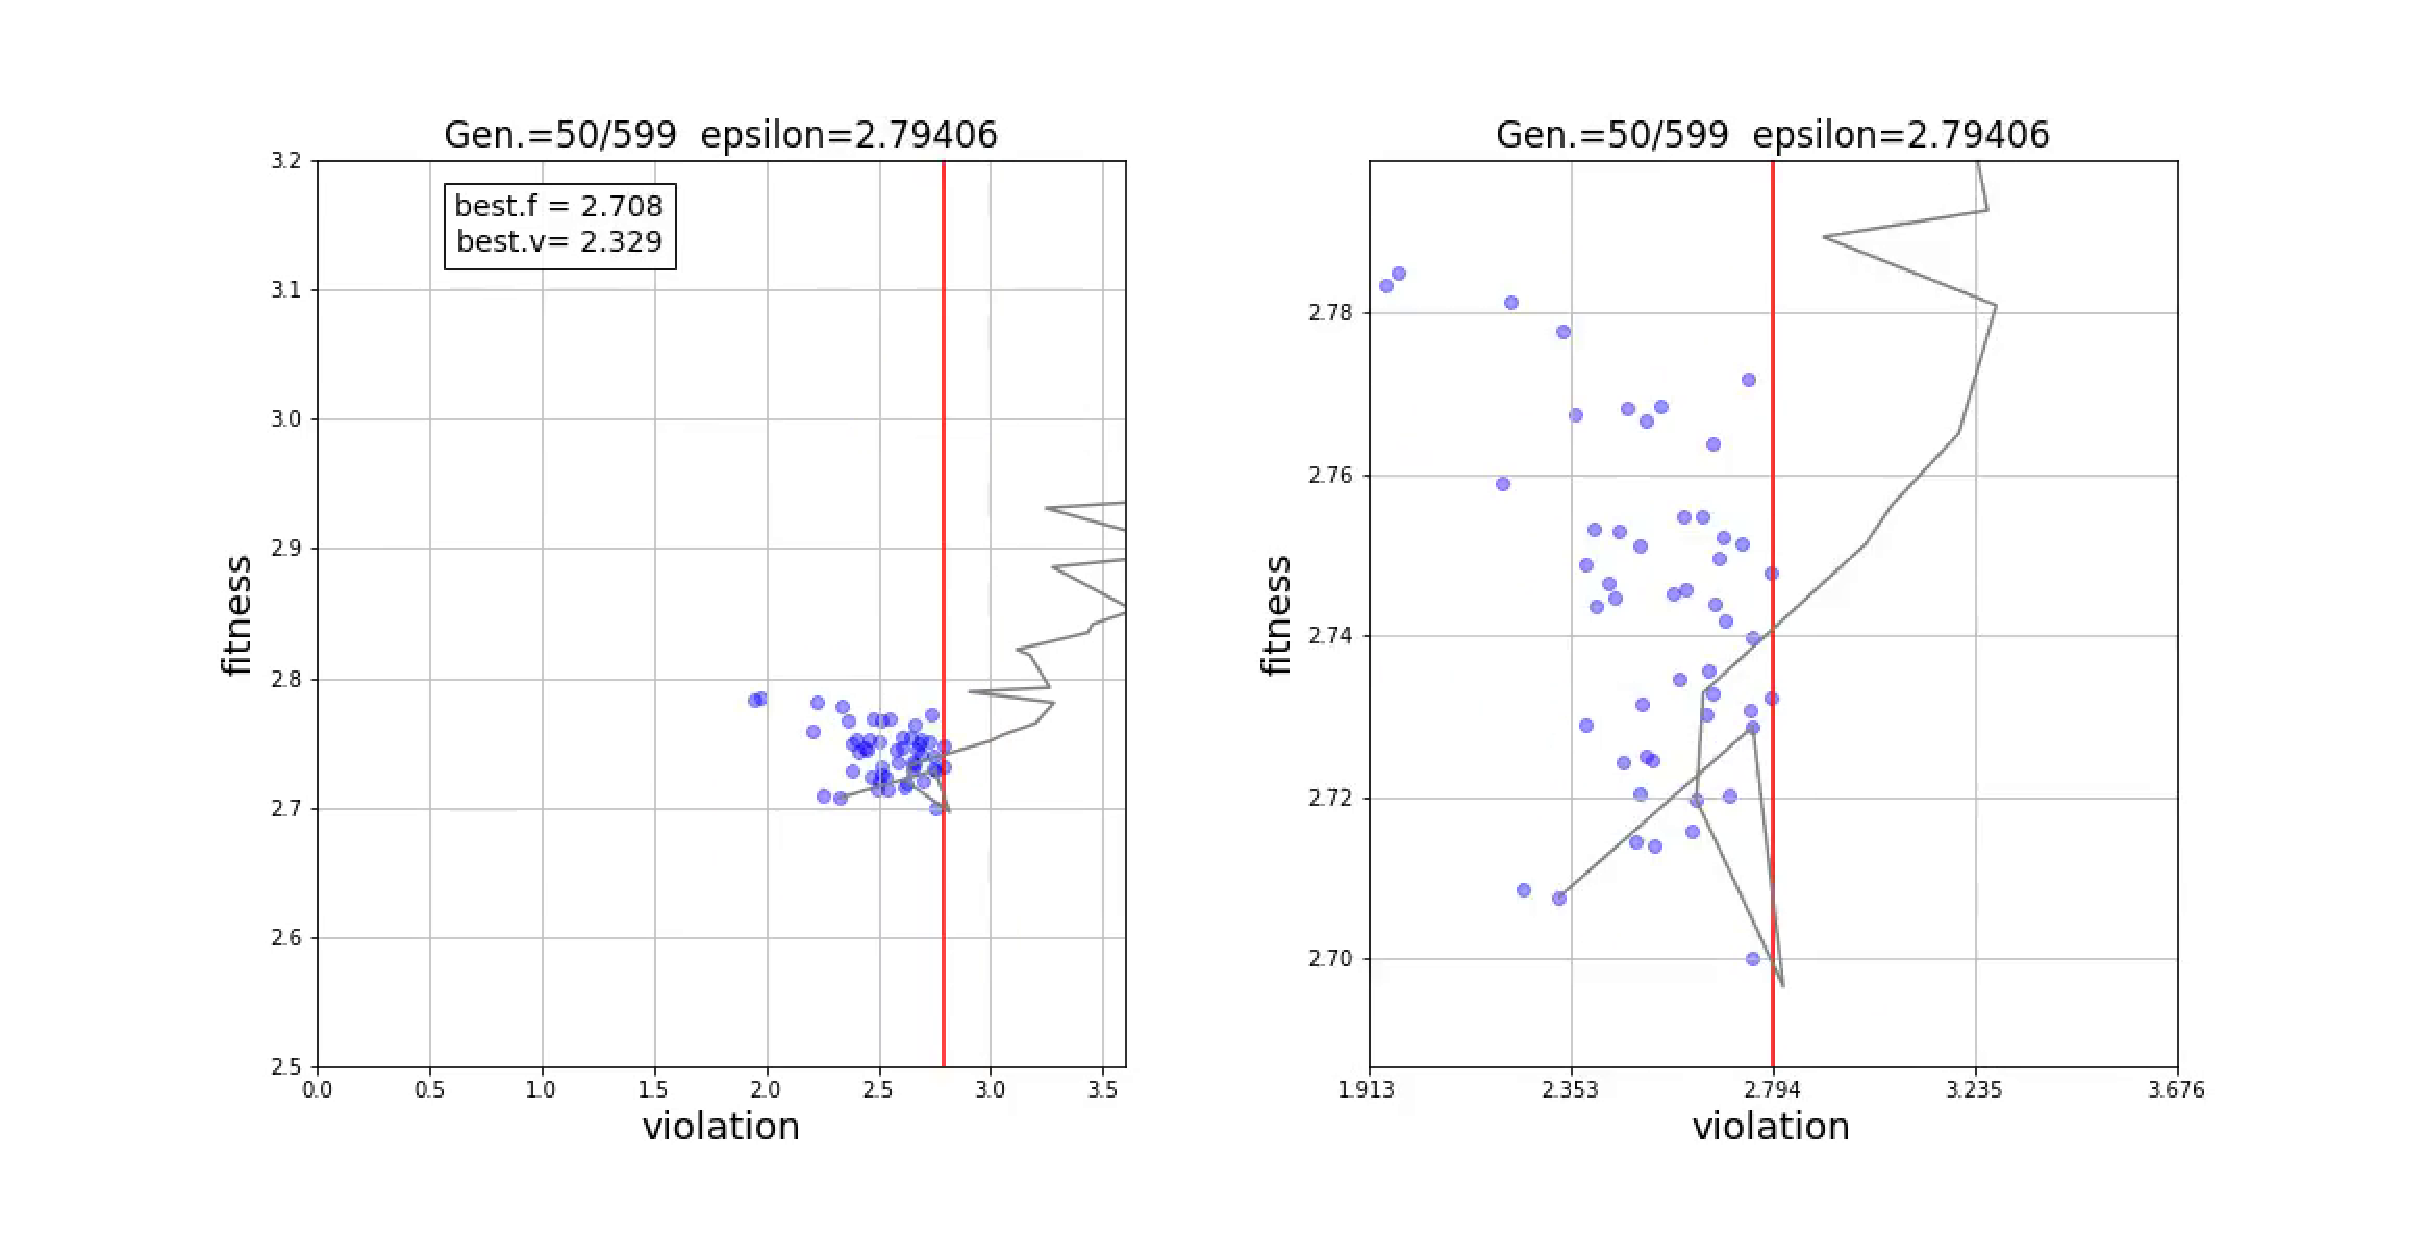
\includegraphics[width=.9\linewidth]{fig2/top_rate=0.9,50.eps}
  \caption{k=0.9,50世代}
\label{fig2:graph8}
\end{figure}
\begin{figure}[htbp]
  \centering
  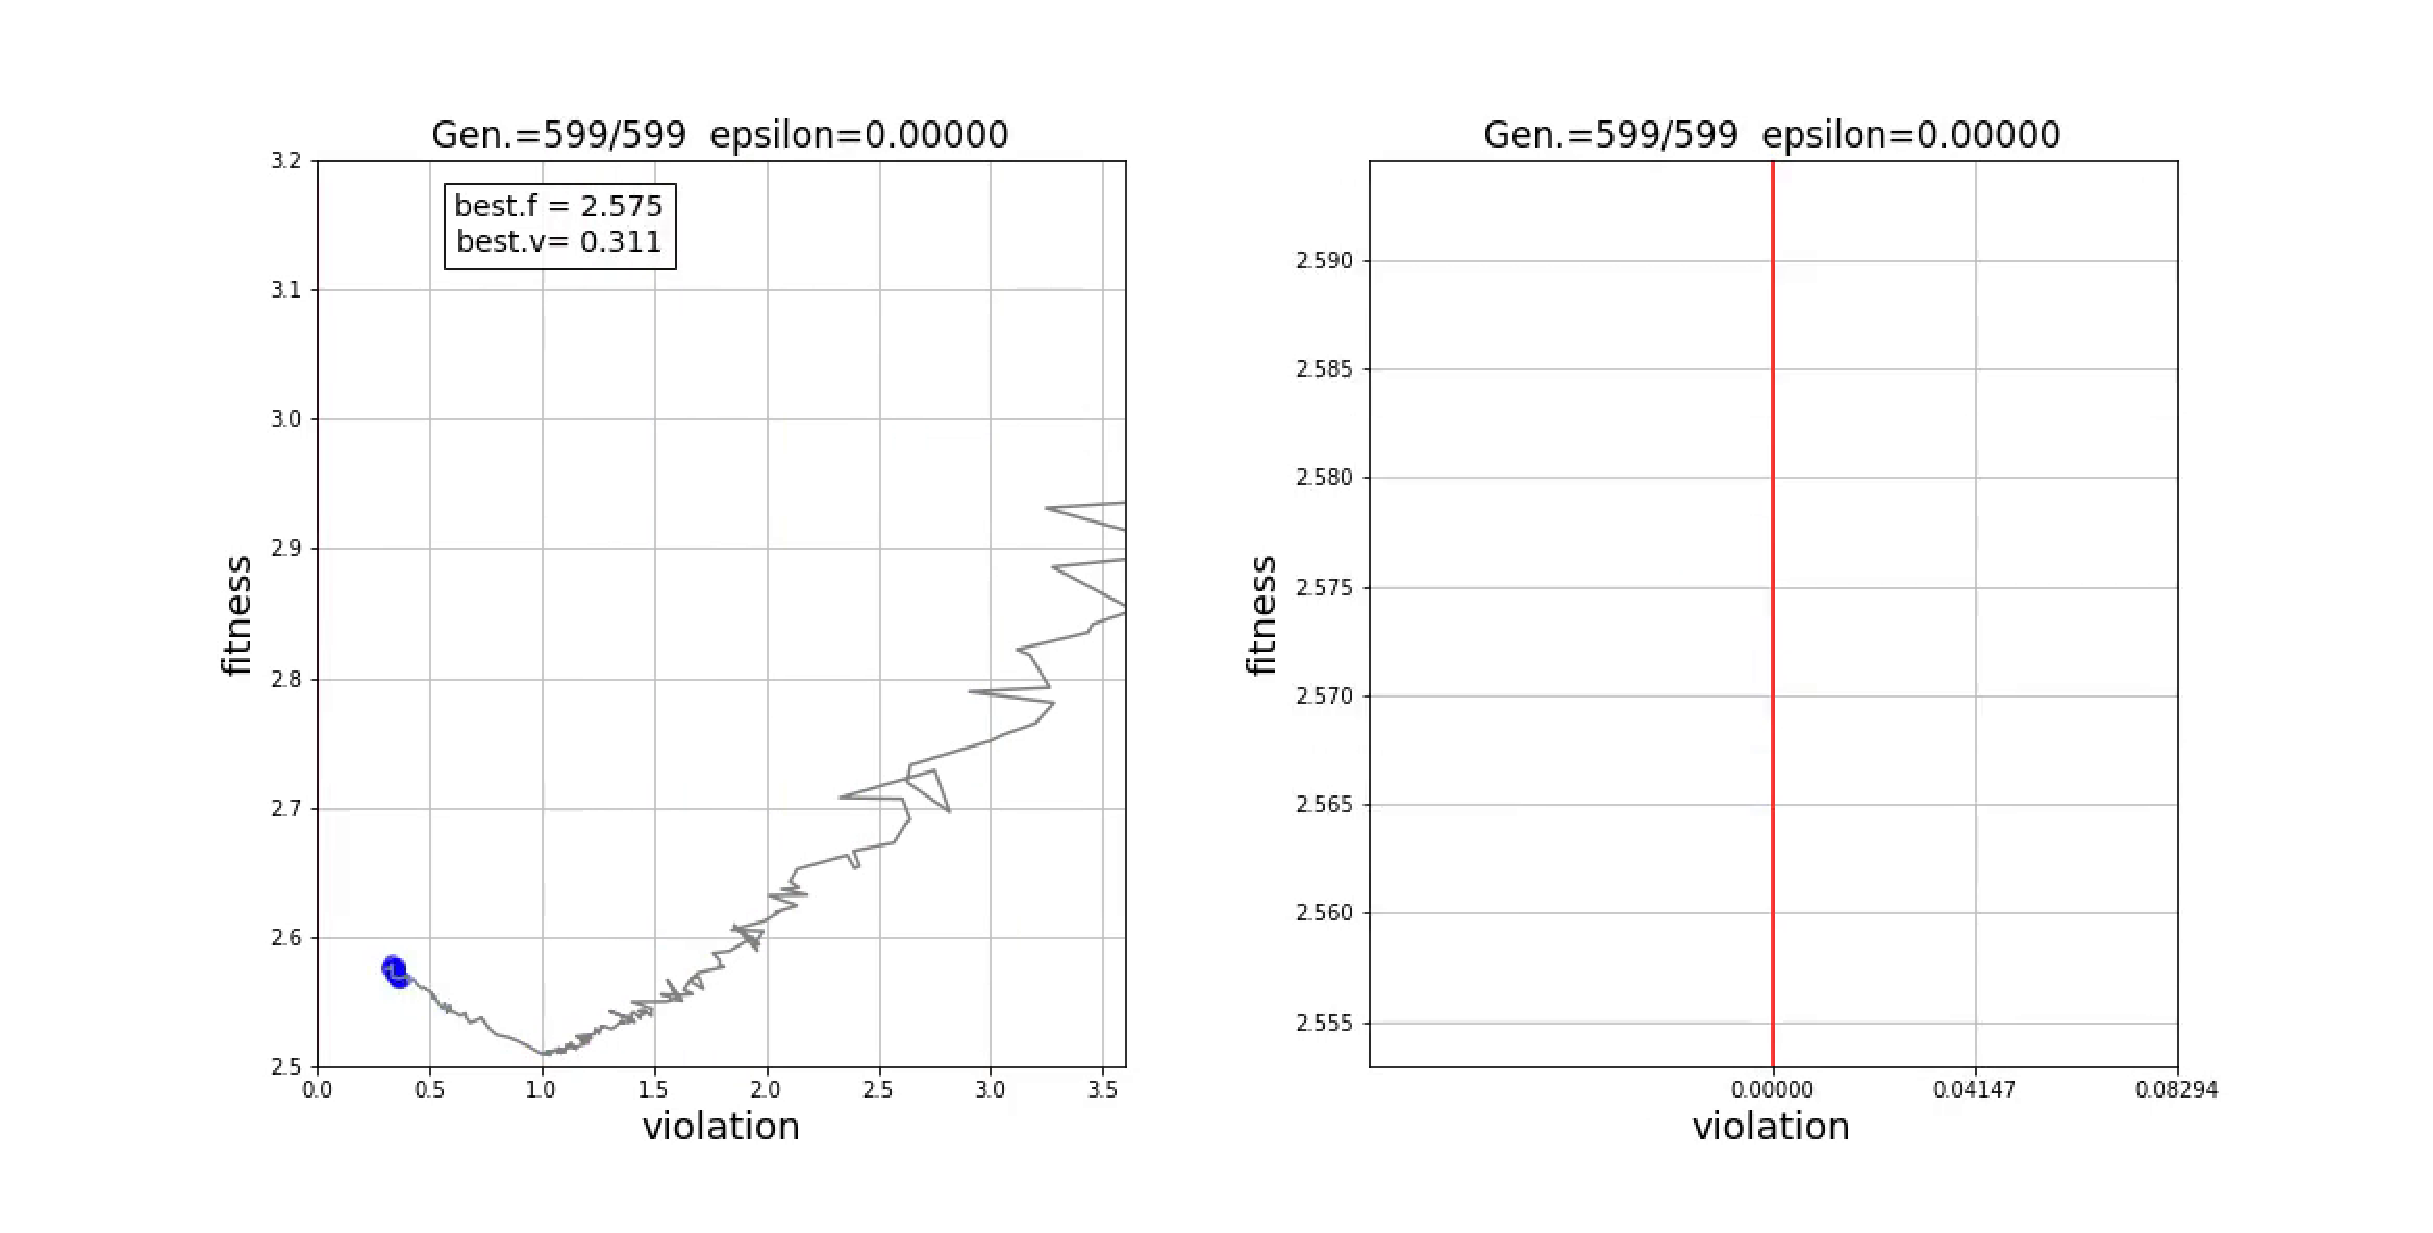
\includegraphics[width=.9\linewidth]{fig2/top_rate=0.9,600.eps}
  \caption{k=0.9,600世代}
\label{fig2:graph9}
\end{figure}
今回の提案手法では、少なくとも0世代から200世代までに制約を満たす個体を得ることができ探索は速い。図\ref{fig2:graph4}、図\ref{fig2:graph5}では、目的関数値と制約逸脱度の良い個体をバランスよく探索できているといえる。

k=0.5でε制約を満たしている個体の数を全体の5割で固定している図\ref{fig2:graph6}、図\ref{fig2:graph7}では、個体集団が急速に制約を満たすような動きをする。これは、ε制約を満たしていない個体が進化しやすいことから、ε制約を満たしていない個体が多すぎると個体集団が制約を満たすような動きをすると考える。

k=0.9でε制約を満たしている個体の数を全体の9割で固定している図\ref{fig2:graph8}、図\ref{fig2:graph9}では、個体集団が急速に目的関数値の良い個体の探索を進める。これは、ε制約を満たしている個体の数が多すぎる事から、目的関数値の良い個体へと個体集団が進化してしまうと考える。

上記の結果より、ε制約を満たしている個体の数と満たしていない個体の数の割合によって個体集団の動きに大きく影響が与えられるので、目的関数値と制約逸脱度をバランスよく改善できるようパラメータkを設定しなければいけない。また、上記でのkの値は、個体数の変化によっても変わってくるので、とても難しいパラメータであるといえる。

\section{探索終盤でのF、CRの変更}
pbest戦略、パレートランク戦略を実行していくなかで、ベースベクトルをそれぞれ設定した個体群から選ぶことになり、探索終盤において個体集団の動きが収束していく傾向がみられた。ここで、探索終盤でF、CRに初期値よりも大きい値を与えることで、差分ベクトルの拡大によって生成した変異ベクトルへ更新、またその変異ベクトルの影響を大きくすることで個体集団に多様性を与える。

提案手法にpbest戦略、パレートランク戦略を導入したものの変更前と変更後の最適解を表\ref{tbl:MLP5}で示す。各初期値は6.3節で使用したパラメータを使用しk=0.8とする。また、パラメータF,CRはF=0.5,CR=0.9に変更する。

\begin{table}[htbp]
\begin{center}
\caption{探索終盤でF,CR変更による最適解}
\label{tbl:MLP5}
\begin{tabular}{|l|c|c|}
\hline
  & pbest戦略 & パレートランク戦略 \\ \hline
変更前 & 2.59544&  2.58546       \\ \hline
εレベル=0時変更 & 2.59965 &  2.58207    \\ \hline 
εレベル=0.05時変更 & 2.59532 &  2.58156    \\ \hline
\end{tabular}
\end{center}
\end{table}
pbest戦略では、パラメータ変更をするタイミングで最適解に統一性は見られなかったが、どちらの戦略でも改善されたといえる。εレベル=0.05時の方が良い最適解が得られたことについては、パラメータ変更のタイミングを早くすることで、個体集団の多様性を少しでも保つことができ、より良い進化ができたと考える。

\bibliography{btxsample}
\bibliographystyle{jplain}

%欧文用	和文用	特徴
%plain	jplain	参考文献をアルファベット順で出力する
%unsrt	junsrt	参考文献を引用された順で出力する

\section{参考文献}
[1]ε制約法とパレート的アプローチを用いたDifferential Evolutionによる複数車種車両の同時最適化 著者:串田淳一、原章、高濱徹行 出版:進化計算学会論文誌 URL:https://ci.nii.ac.jp/naid/130007797834\\

[2]難易度による制約分割を用いた段階的制約充足法の適用に関する検討著者:丹羽健斗、古川大弘 出版:第14回進化計算学会研究会 URL:https://kaken.nii.ac.jp/grant/KAKENHI-PROJECT-15K00336/


\begin{table*}[htbp]
\caption{表の例(表を1段組で表示)}
\label{results}
\begin{center}
\begin{tabular}{|c|c|c|c|c|c|c|} \hline
model & \multicolumn{2}{c|}{LeNet} & \multicolumn{2}{c|}{ResNet} & \multicolumn{2}{c|}{DenseNet} \\\hline
\#pixels & 1 & 3 & 1 & 3 & 1 & 3 \\\hline
$\varepsilon$JADE $L=0.1$ & 7.0\% & 13.0\% & 5.5\% & 12.0\% & 5.5\%& 11.0\% \\\hline
$\varepsilon$JADE $L=0.2$ & 20.0\% & 35.0\% & 16.5\% & 30.0\% & 11.0\% & 26.0\% \\\hline
$\varepsilon$JADE $L=0.3$ & 28.5\% & 52.0\% & 22.0\% & 48.0\% & 15.5\% & 45.5\% \\\hline
$\varepsilon$JADE $L=1.0$ & 57.5\% & 91.5\% & 33.0\% & 80.5\% & 25.0\% & 67.5\% \\\hline
\hline
random $L=1.0$ & 51.5\% & 68.0\% & 28.5\% & 47.0\% & 20.0\% & 35.5\% \\\hline

\end{tabular}
\end{center}
\end{table*}


\begin{algorithm}[htbp]
\DontPrintSemicolon
  
$j_r=$select randomly from $[1,D]$;
 
\For{$ j = 1$ \KwTo $D$} {

    \eIf{$ {\rm rand}(0,1) < CR$  {\rm or} $j=j_r  $}{
    $ u_{i,j}$=  $v_{i,j}$;
    }
    {
    $u_{i,j}$=  $x_{i,j}$;
    }

}

\caption{binomial crossover}         
\label{Alg:bin}   
\end{algorithm}



\end{document}